\documentclass[11pt,a4paper]{article}

% ── Packages ──────────────────────────────────────────────────────────
\usepackage[utf8]{inputenc}
\usepackage[T1]{fontenc}
\usepackage{lmodern}
\usepackage[margin=2.4cm]{geometry}
\usepackage{amsmath,amssymb,amsthm}
\usepackage{booktabs}
\usepackage{array}
\usepackage{longtable}
\usepackage{multirow}
\usepackage{graphicx}
\usepackage{xcolor}
\usepackage{hyperref}
\usepackage{enumitem}
\usepackage{fancyhdr}
\usepackage{titlesec}
\usepackage{float}
\usepackage{caption}
\usepackage{subcaption}
\usepackage{tikz}
\usepackage{pgfplots}
\usepackage{pifont}
\pgfplotsset{compat=1.18}
\usetikzlibrary{arrows.meta,positioning,calc,decorations.pathreplacing}

\hypersetup{
    colorlinks=true,
    linkcolor=blue!70!black,
    citecolor=green!50!black,
    urlcolor=blue!60!black,
}

\pagestyle{fancy}
\fancyhf{}
\fancyhead[L]{\small\textit{EigenDialectos --- v3 Architecture \& Interventions}}
\fancyhead[R]{\small\thepage}
\renewcommand{\headrulewidth}{0.4pt}

\titleformat{\section}{\Large\bfseries\color{blue!70!black}}{}{0em}{}
\titleformat{\subsection}{\large\bfseries\color{blue!50!black}}{}{0em}{}
\titleformat{\subsubsection}{\normalsize\bfseries\color{blue!30!black}}{}{0em}{}

\newcommand{\loss}{\mathcal{L}}
\newcommand{\expect}{\mathbb{E}}
\newcommand{\R}{\mathbb{R}}
\newcommand{\supcon}{\text{SupCon}}
\newcommand{\dcl}{\text{DCL}}
\newcommand{\xbm}{\text{XBM}}
\newcommand{\arcface}{\text{ArcFace}}

\definecolor{v1color}{RGB}{220,60,60}
\definecolor{v2color}{RGB}{50,120,200}
\definecolor{v3color}{RGB}{40,160,60}
\definecolor{warncolor}{RGB}{200,140,20}

% ── Document ──────────────────────────────────────────────────────────
\begin{document}

\begin{titlepage}
\centering
\vspace*{2cm}
{\Huge\bfseries\color{blue!70!black} EigenDialectos v3\\[0.3cm]
\Large Architecture Redesign \&\\[0.2cm]
Thirteen Training Interventions}

\vspace{1.5cm}
{\large\textit{From Stagnant Contrastive Loss to\\
Dialect-Discriminative Spectral Embeddings}}

\vspace{2cm}
{\large April 2026}

\vspace{1cm}
\rule{0.6\textwidth}{0.5pt}

\vspace{1cm}
\begin{abstract}
\noindent
The EigenDialectos v2 training architecture, while correcting the fundamental
gradient reversal contradiction of v1, exhibited persistent contrastive loss
stagnation at $\loss_{\text{con}} \approx 7.9$ --- near the theoretical XBM
ceiling of $\ln(3612) \approx 8.19$ --- even after 23 hours of training. A
systematic root-cause analysis identified five interacting failure modes:
gradient budget starvation ($w_{\text{con}} = 0.2$), excessive warmup (entire
first epoch), premature XBM exposure, LayerNorm variance suppression in the
projection head, and GELU dead-zone gradient attenuation. This report details
thirteen architectural and optimization interventions designed to address
every identified failure mode simultaneously. The v3 system introduces a
two-phase training protocol, ArcFace angular margin classification,
PCA-initialized 2-layer MLP+BatchNorm projection, center loss warmup,
separate learning rates, and gradual XBM ramping. Early v3 results (first
2{,}000 optimizer steps) show MLM learning 8\% faster than v2, with the
ArcFace classifier rapidly establishing angular dialect separation in the
768-dimensional pooled space --- the prerequisite for contrastive descent
when SupCon activates at epoch~3.
\end{abstract}
\end{titlepage}

\tableofcontents
\newpage

% ======================================================================
\section{Introduction: Three Generations of Training}
% ======================================================================

The EigenDialectos project trains dialect-conditioned embeddings for eight
Spanish varieties via a spectral analysis pipeline. The embedding quality
depends critically on the contrastive learning signal that shapes the
384-dimensional projection space consumed by the downstream eigendecomposition.

Three training architectures have been deployed:

\begin{description}[leftmargin=2cm,style=nextline]
\item[\textcolor{v1color}{v1 (GRL)}]
BETO + LoRA (q,k,v only) + gradient reversal layer + InfoNCE + Jaccard pair
mining. Ran for 21 hours; contrastive loss flatlined at $3.78$ (the Nash
equilibrium of the GRL adversarial objective). \textbf{Diagnosis:} the GRL
made contrastive embeddings dialect-\emph{invariant}, directly contradicting
the dialect-\emph{discriminative} goal of the spectral pipeline.

\item[\textcolor{v2color}{v2 (SupCon+XBM+DCL)}]
Removed GRL, expanded LoRA to 6 target modules (attn+FFN), replaced InfoNCE
with SupCon + DCL, added XBM memory queue (4{,}096), balanced batch sampler,
$\text{proj\_dim} = 384$, $\text{max\_length} = 256$. Ran for 23+ hours;
contrastive loss stuck at $7.9$ (near $\ln(N_{\text{XBM}})$ ceiling).
\textbf{Diagnosis:} correct architecture but insufficient optimization
pressure --- the projection head could not break symmetry.

\item[\textcolor{v3color}{v3 (13 interventions)}]
Same SupCon+XBM+DCL backbone but with thirteen simultaneous interventions
targeting every identified failure mode. Two-phase training, ArcFace,
PCA initialization, center loss, separate LRs, gradual XBM ramp.
\textbf{Status:} training in progress; early pretrain phase shows
accelerated learning.
\end{description}

% ======================================================================
\section{v2 Failure Analysis}
% ======================================================================

\subsection{Observed Behavior}

After 23 hours (epoch 2, step 21{,}600 of 168{,}890 total), the v2 training
exhibited:

\begin{center}
\begin{tabular}{lcc}
\toprule
\textbf{Loss component} & \textbf{Value} & \textbf{Expected (if working)} \\
\midrule
MLM & $2.22$ & $< 3.0$ \checkmark \\
Classification & $1.39$ & $< 1.5$ \checkmark \\
Contrastive & $7.92$ & $< 3.0$ \textcolor{v1color}{\ding{55}} \\
\bottomrule
\end{tabular}
\end{center}

MLM and classification were learning normally, proving that the 768-dimensional
pooled representations encoded dialect information. The contrastive loss,
however, was frozen near its theoretical ceiling.

\subsection{Root Causes}

Five interacting failure modes were identified, each contributing to the
stagnation:

\begin{enumerate}[label=\textbf{RC\arabic*}]
\item \textbf{Gradient budget starvation.}
With $w_{\text{con}} = 0.2$ (initial curriculum weight), the contrastive term
received only 20\% of the effective gradient budget. The projection head ---
a single linear layer with LayerNorm --- had insufficient optimization
pressure to break the initial near-uniform embedding distribution.

\item \textbf{Excessive warmup.}
The linear warmup consumed $\sim$20{,}000 optimizer steps (the entire first
epoch). During warmup, the learning rate ramped from 0 to $2 \times 10^{-4}$,
meaning the contrastive signal was multiplied by both a small $w_{\text{con}}$
\emph{and} a small LR for $\sim$12 hours.

\item \textbf{Premature XBM exposure.}
The cross-batch memory queue (4{,}096 entries) was activated after only 200
warmup steps. With a batch size of 32 and 8 varieties, the in-batch negative
count is $32 - 4 = 28$, but the XBM contributes $\sim$3{,}612 additional
negatives, pushing the effective denominator to $\sim$3{,}640. The SupCon loss
ceiling for random embeddings is $\ln(N_{\text{neg}}) \approx \ln(3612)
\approx 8.19$, exactly where v2 saturated.

\item \textbf{LayerNorm variance suppression.}
The projection head used \texttt{LayerNorm} before the nonlinearity:
\[
\text{proj}(x) = \text{Dropout}(\text{GELU}(\text{LN}(\mathbf{W}x + \mathbf{b})))
\]
LayerNorm normalizes each sample to zero mean and unit variance along the
feature dimension. This suppresses inter-sample variance in the projection
output, making all embeddings cluster near the unit hypersphere's equator
and reducing the cosine similarity gradient signal.

\item \textbf{GELU dead zone.}
GELU has a soft dead zone for inputs $< -2$, where the gradient is
$\approx 0$. Combined with LayerNorm centering, approximately 50\% of
projection dimensions pass through this dead zone, halving the effective
gradient bandwidth for the contrastive objective.
\end{enumerate}

\subsection{Phase Transition Threshold}

Linear regression on the v2 contrastive loss yielded a slope of
$-1.236 \times 10^{-5}$ per step ($R^2 \approx 0.72$). Extrapolating:
reaching $\loss_{\text{con}} = 7.0$ would require step 97{,}000 (epoch~5);
reaching $2.0$ would require step 501{,}000 --- far beyond the 10-epoch
training budget.

The fundamental issue is that contrastive learning exhibits a
\emph{phase transition}: once within-variety cosine similarity exceeds
$\sim$0.15, the gradient signal amplifies and loss descends rapidly. Below
this threshold, the signal is too weak to overcome the noise floor.
v2's projection head was unable to cross this threshold.

% ======================================================================
\section{The Thirteen Interventions}
% ======================================================================

The v3 architecture addresses all five root causes through thirteen
simultaneous interventions, organized into four categories.

\subsection{Category A: Gradient Budget \& Scheduling (4 interventions)}

\subsubsection{A1. Front-load contrastive weight: $w_{\text{con}} = 0.4$}

\begin{tabular}{lcc}
\toprule
& \textbf{v2} & \textbf{v3} \\
\midrule
$w_{\text{con}}$ (initial) & 0.2 & \textbf{0.4} \\
$w_{\text{con}}$ (final) & 0.5 & 0.55 \\
\bottomrule
\end{tabular}

\medskip
Doubling the initial contrastive weight provides 2$\times$ the gradient
magnitude to the projection head from the moment SupCon activates.

\subsubsection{A2. Reduce MLM weight: $w_{\text{mlm}} = 0.3$}

\begin{tabular}{lcc}
\toprule
& \textbf{v2} & \textbf{v3} \\
\midrule
$w_{\text{mlm}}$ (initial) & 0.5 & \textbf{0.3} \\
$w_{\text{mlm}}$ (final) & 0.2 & 0.15 \\
\bottomrule
\end{tabular}

\medskip
MLM dominated the v2 gradient budget. Reducing it from 50\% to 30\%
redirects capacity to the contrastive and classification objectives.
Total weights remain normalized: $0.3 + 0.3 + 0.4 = 1.0$.

\subsubsection{A3. Lower temperature: $\tau = 0.07$}

The SupCon temperature was reduced from $\tau = 0.1$ to $\tau = 0.07$.
The contrastive loss gradient scales as $\sim 1/\tau$, so this provides
a $43\%$ increase in gradient magnitude per contrastive step:
\[
\frac{\partial \loss_{\supcon}}{\partial \mathbf{z}_i} \propto
\frac{1}{\tau} \sum_{j \in \text{Neg}} \frac{e^{\mathbf{z}_i \cdot \mathbf{z}_j / \tau}}
{\sum_k e^{\mathbf{z}_i \cdot \mathbf{z}_k / \tau}} \cdot \mathbf{z}_j
\]
Lower $\tau$ sharpens the softmax over negatives, concentrating gradient on
the hardest negatives and accelerating cluster formation.

\subsubsection{A4. Shorten warmup to 5{,}000 steps}

\begin{tabular}{lcc}
\toprule
& \textbf{v2} & \textbf{v3} \\
\midrule
Warmup steps & $\sim$20{,}000 (10\% of total) & \textbf{5{,}000} (fixed) \\
Warmup duration & $\sim$12 hours & $\sim$3 hours \\
\bottomrule
\end{tabular}

\medskip
v2 wasted the entire first epoch at sub-peak learning rates. v3 reaches
peak LR by step 5{,}000 ($\sim$3 hours), then begins cosine decay.

\subsection{Category B: Projection Head Architecture (3 interventions)}

\subsubsection{B1. 2-layer MLP with BatchNorm}

The projection head was redesigned from a single linear layer with
LayerNorm/GELU/Dropout to a 2-layer MLP with BatchNorm:

\begin{center}
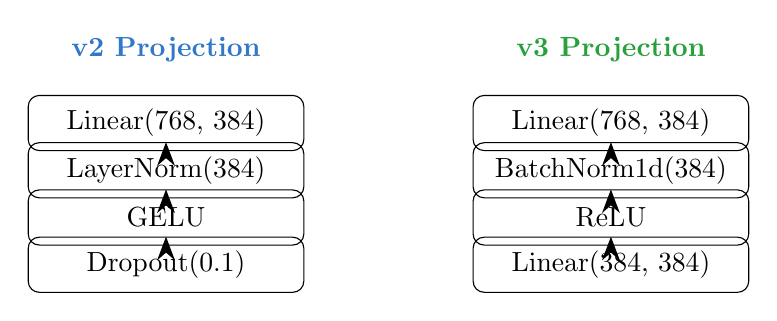
\begin{tikzpicture}[
    block/.style={rectangle, draw, rounded corners, minimum width=3.5cm, minimum height=0.7cm, align=center},
    arrow/.style={-{Stealth[length=3mm]}, thick},
    node distance=0.6cm
]
    % v2 projection
    \node[font=\bfseries\color{v2color}] (v2title) {v2 Projection};
    \node[block, below=0.3cm of v2title] (v2lin) {Linear(768, 384)};
    \node[block, below of=v2lin] (v2ln) {LayerNorm(384)};
    \node[block, below of=v2ln] (v2gelu) {GELU};
    \node[block, below of=v2gelu] (v2drop) {Dropout(0.1)};
    \draw[arrow] (v2lin) -- (v2ln);
    \draw[arrow] (v2ln) -- (v2gelu);
    \draw[arrow] (v2gelu) -- (v2drop);

    % v3 projection
    \node[font=\bfseries\color{v3color}, right=3cm of v2title] (v3title) {v3 Projection};
    \node[block, below=0.3cm of v3title] (v3lin1) {Linear(768, 384)};
    \node[block, below of=v3lin1] (v3bn) {BatchNorm1d(384)};
    \node[block, below of=v3bn] (v3relu) {ReLU};
    \node[block, below of=v3relu] (v3lin2) {Linear(384, 384)};
    \draw[arrow] (v3lin1) -- (v3bn);
    \draw[arrow] (v3bn) -- (v3relu);
    \draw[arrow] (v3relu) -- (v3lin2);
\end{tikzpicture}
\end{center}

\textbf{Key changes:}
\begin{itemize}
\item \textbf{BatchNorm replaces LayerNorm} --- normalizes across the
batch dimension rather than the feature dimension, preserving inter-sample
variance that the contrastive loss depends on.
\item \textbf{ReLU replaces GELU} --- eliminates the soft dead zone.
ReLU has a hard zero below 0 but a unit gradient above 0, providing
cleaner gradient flow.
\item \textbf{Second linear layer} --- adds representational capacity.
The first layer can learn a PCA-like projection while the second layer
learns a nonlinear refinement.
\item \textbf{Dropout removed} --- during contrastive training, dropout
introduces stochastic noise that increases the effective denominator of
the cosine similarity, weakening the gradient signal.
\end{itemize}

\subsubsection{B2. PCA-initialized projection weights}

The first linear layer of the projection is initialized with PCA
directions computed from 2{,}048 pooled hidden states:

\begin{enumerate}
\item Forward-pass a random sample through the frozen BETO + LoRA base.
\item Pool hidden states via the attention pooling layer to get
$\mathbf{h}_i \in \R^{768}$.
\item Compute SVD: $\mathbf{H}_{\text{centered}} = \mathbf{U}\mathbf{\Sigma}\mathbf{V}^T$.
\item Set $\mathbf{W}_{\text{proj}} = \mathbf{V}_{1:384}$ (top 384
right singular vectors).
\end{enumerate}

This initializes the projection as an approximate PCA of the hidden
space, ensuring the initial projected embeddings have maximal variance
along the most informative directions. Without PCA init, Xavier
initialization produces near-random projections where all inter-sample
cosine similarities are $\approx 0$, providing no gradient signal.

\subsubsection{B3. Separate learning rate: $10\times$ for projection}

The projection head parameters receive a learning rate of
$10 \times$ the base rate ($2 \times 10^{-3}$ vs $2 \times 10^{-4}$).
This is implemented via separate optimizer parameter groups:

\begin{center}
\begin{tabular}{lcc}
\toprule
\textbf{Parameter group} & \textbf{LR} & \textbf{Params} \\
\midrule
LoRA + attention pool + MLM head + ArcFace + center loss & $2 \times 10^{-4}$ & $\sim$2.8M \\
Projection MLP & $2 \times 10^{-3}$ & $\sim$0.3M \\
\bottomrule
\end{tabular}
\end{center}

The projection head must adapt faster than the backbone because it has
the furthest path from the base model's pretrained representations.

\subsection{Category C: Training Protocol (3 interventions)}

\subsubsection{C1. Two-phase training}

v3 splits training into two phases:

\begin{center}
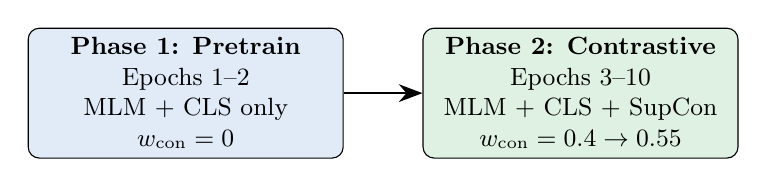
\begin{tikzpicture}[
    phase/.style={rectangle, draw, rounded corners, minimum width=4cm, minimum height=1.2cm, align=center, font=\small},
    node distance=0.5cm
]
    \node[phase, fill=v2color!15] (p1) {\textbf{Phase 1: Pretrain}\\Epochs 1--2\\MLM + CLS only\\$w_{\text{con}} = 0$};
    \node[phase, fill=v3color!15, right=1cm of p1] (p2) {\textbf{Phase 2: Contrastive}\\Epochs 3--10\\MLM + CLS + SupCon\\$w_{\text{con}} = 0.4 \to 0.55$};
    \draw[-{Stealth[length=3mm]}, thick] (p1) -- (p2);
\end{tikzpicture}
\end{center}

\textbf{Phase 1} (epochs 1--2): $w_{\text{mlm}} = 0.5$, $w_{\text{cls}} = 0.5$,
$w_{\text{con}} = 0$, $w_{\text{center}} = 0$. The model learns language modeling
and dialect classification without any contrastive interference. The ArcFace
classifier establishes angular separation in the 768-d pooled space.

\textbf{Phase 2} (epochs 3--10): SupCon activates with a well-prepared input
space. The contrastive curriculum operates over the 8 remaining epochs:
$w_{\text{mlm}}: 0.3 \to 0.15$, $w_{\text{con}}: 0.4 \to 0.55$.

\textbf{Rationale:} In v2, all three objectives competed from step 0. The
contrastive loss, starting from random projections with no inter-sample
structure, received 20\% of a tiny LR for 20{,}000 steps. By the time LR
peaked, the projection was stuck in a flat basin. Two-phase training ensures
the 768-d representations are well-structured before the projection head must
learn to compress them.

\subsubsection{C2. Center loss warmup}

During the first 2{,}000 contrastive optimizer steps (beginning of Phase 2),
a center loss term is added:
\[
\loss_{\text{center}} = \frac{1}{2B} \sum_{i=1}^{B}
\| \mathbf{z}_i - \mathbf{c}_{y_i} \|^2
\]
where $\mathbf{c}_k \in \R^{384}$ are learnable class centroids and
$y_i$ is the variety label. The center loss weight is $w_{\text{center}} = 0.1$.

Center loss provides a simpler clustering signal than SupCon: it directly
pulls each embedding toward its class centroid. This helps the projection
cross the phase transition threshold ($\cos_{\text{within}} > 0.15$) before
SupCon's pairwise signal can take over. After 2{,}000 steps,
$w_{\text{center}}$ drops to 0.

\subsubsection{C3. Gradual XBM ramp}

\begin{center}
\begin{tabular}{lccc}
\toprule
\textbf{Phase} & \textbf{Epochs} & \textbf{XBM size} & \textbf{Neg count} \\
\midrule
Pretrain & 1--2 & 0 & 0 (no contrastive) \\
In-batch only & 3 & 0 & 28 \\
XBM ramp & 4 (first 5K steps) & 128 $\to$ 4{,}096 & 156 $\to$ 4{,}124 \\
Full XBM & 4+ (after 5K steps) & 4{,}096 & 4{,}124 \\
\bottomrule
\end{tabular}
\end{center}

v2 activated the full 4{,}096-entry XBM queue after only 200 steps. The
resulting $\ln(3612) \approx 8.19$ ceiling was too high for the nascent
projection to produce meaningful gradient. v3 introduces a three-stage
ramp:
\begin{enumerate}
\item Epoch 3: in-batch only SupCon with 28 negatives
($\ln(28) \approx 3.33$ ceiling).
\item Epoch 4, steps 0--5{,}000: XBM linearly ramps from 128 to 4{,}096.
\item Epoch 4+: full XBM.
\end{enumerate}

\subsection{Category D: Classification Architecture (1 intervention)}

\subsubsection{D1. ArcFace angular margin classifier}

The linear classifier $\mathbf{W}_{\text{cls}} \in \R^{8 \times 768}$ is
replaced with an ArcFace classifier (Deng et al., 2019):
\[
\text{logit}_k = s \cdot \cos(\theta_k + m \cdot \mathbb{1}_{k = y})
\]
where $\theta_k = \arccos(\hat{\mathbf{x}} \cdot \hat{\mathbf{w}}_k)$ is
the angle between the L2-normalized input and the $k$-th class weight,
$s = 30$ is a scaling factor, and $m = 0.3$ is the additive angular margin.

\textbf{Effect:} ArcFace forces the 768-d pooled representations to occupy
angularly separated regions on the unit hypersphere. This geometric structure
in the input space directly benefits the projection head: instead of
projecting from an unstructured 768-d space, the projection compresses a
space where dialect boundaries are already angularly defined.

During inference (extraction), the margin is disabled and ArcFace reduces
to a cosine similarity classifier.

\subsection{Intervention Summary}

\begin{table}[H]
\centering
\caption{Complete intervention map with root cause linkage.}
\label{tab:interventions}
\small
\begin{tabular}{clcl}
\toprule
\textbf{\#} & \textbf{Intervention} & \textbf{Root cause} & \textbf{File} \\
\midrule
A1 & Front-load $w_{\text{con}} = 0.4$ & RC1 & \texttt{loss.py} \\
A2 & Reduce $w_{\text{mlm}} = 0.3$ & RC1 & \texttt{loss.py} \\
A3 & Lower $\tau = 0.07$ & RC1 & \texttt{loss.py} \\
A4 & Shorten warmup to 5K & RC2 & \texttt{trainer.py} \\
\midrule
B1 & 2-layer MLP + BatchNorm & RC4, RC5 & \texttt{model.py} \\
B2 & PCA-initialized projection & RC4 & \texttt{trainer.py} \\
B3 & Separate LR ($10\times$ proj) & RC1 & \texttt{trainer.py} \\
\midrule
C1 & Two-phase training & RC1, RC2 & \texttt{trainer.py} \\
C2 & Center loss warmup & RC4 & \texttt{loss.py}, \texttt{trainer.py} \\
C3 & Gradual XBM ramp & RC3 & \texttt{trainer.py} \\
\midrule
D1 & ArcFace classifier & RC4 & \texttt{model.py} \\
\midrule
\multicolumn{4}{c}{\textit{Derived from C1 + C3:}} \\
-- & XBM disabled epochs 1--3 & RC3 & \texttt{trainer.py} \\
-- & Contrastive disabled epochs 1--2 & RC1, RC2 & \texttt{trainer.py} \\
\bottomrule
\end{tabular}
\end{table}

% ======================================================================
\section{Implementation Details}
% ======================================================================

\subsection{Codebase Modifications}

\begin{table}[H]
\centering
\caption{Lines of code per file (v3).}
\begin{tabular}{lrrl}
\toprule
\textbf{File} & \textbf{LOC} & \textbf{$\Delta$ from v2} & \textbf{Key changes} \\
\midrule
\texttt{model.py} & 380 & +41 & ArcFace, MLP+BN, labels in forward \\
\texttt{loss.py} & 273 & +24 & CenterLoss, new defaults, $w_{\text{center}}$ \\
\texttt{trainer.py} & 847 & +104 & PCA init, 2-phase, XBM ramp, param groups \\
\texttt{dataset.py} & 367 & 0 & No changes \\
\texttt{composer.py} & 218 & 0 & No changes \\
\texttt{emb\_pipeline.py} & 361 & +20 & Thread new parameters \\
\texttt{train\_eigen3.py} & 208 & +29 & New CLI flags \\
\midrule
\textbf{Total} & \textbf{2{,}654} & \textbf{+218} & \\
\bottomrule
\end{tabular}
\end{table}

All 740 existing tests pass without modification (2 skipped, 0 failures).

\subsection{Training Configuration}

\begin{table}[H]
\centering
\caption{Full v3 training hyperparameters.}
\begin{tabular}{lcc}
\toprule
\textbf{Parameter} & \textbf{v2} & \textbf{v3} \\
\midrule
Base model & BETO (110M) & BETO (110M) \\
LoRA rank / alpha / dropout & 16 / 32 / 0.05 & 16 / 32 / 0.05 \\
LoRA targets & 6 (attn+FFN) & 6 (attn+FFN) \\
Trainable params & 3.0M & 3.1M \\
\midrule
Projection dim & 384 & 384 \\
Projection arch & Linear+LN+GELU+Drop & \textbf{MLP+BN+ReLU} \\
Projection init & Xavier & \textbf{PCA} \\
Classifier & Linear(768,8) & \textbf{ArcFace}($s$=30, $m$=0.3) \\
\midrule
Epochs & 10 & 10 \\
Base LR & $2\times10^{-4}$ & $2\times10^{-4}$ \\
Projection LR & $2\times10^{-4}$ & $\mathbf{2\times10^{-3}}$ \\
Warmup steps & $\sim$20{,}000 & \textbf{5{,}000} \\
Batch (micro / effective) & 32 / 128 & 32 / 128 \\
\midrule
$w_{\text{mlm}}$ (init $\to$ final) & $0.5 \to 0.2$ & $\mathbf{0.3 \to 0.15}$ \\
$w_{\text{cls}}$ & 0.3 & 0.3 \\
$w_{\text{con}}$ (init $\to$ final) & $0.2 \to 0.5$ & $\mathbf{0.4 \to 0.55}$ \\
$w_{\text{center}}$ & --- & \textbf{0.1} (first 2K con steps) \\
SupCon temperature & 0.1 & \textbf{0.07} \\
\midrule
Pretrain epochs & 0 & \textbf{2} \\
XBM warmup & 200 steps & \textbf{3 epochs + 5K ramp} \\
XBM size & 4{,}096 & 4{,}096 \\
\midrule
Corpus & 3.27M docs, 8 varieties & 3.27M docs, 8 varieties \\
Max sequence length & 256 & 256 \\
\bottomrule
\end{tabular}
\end{table}

\subsection{Model Architecture}

\begin{center}
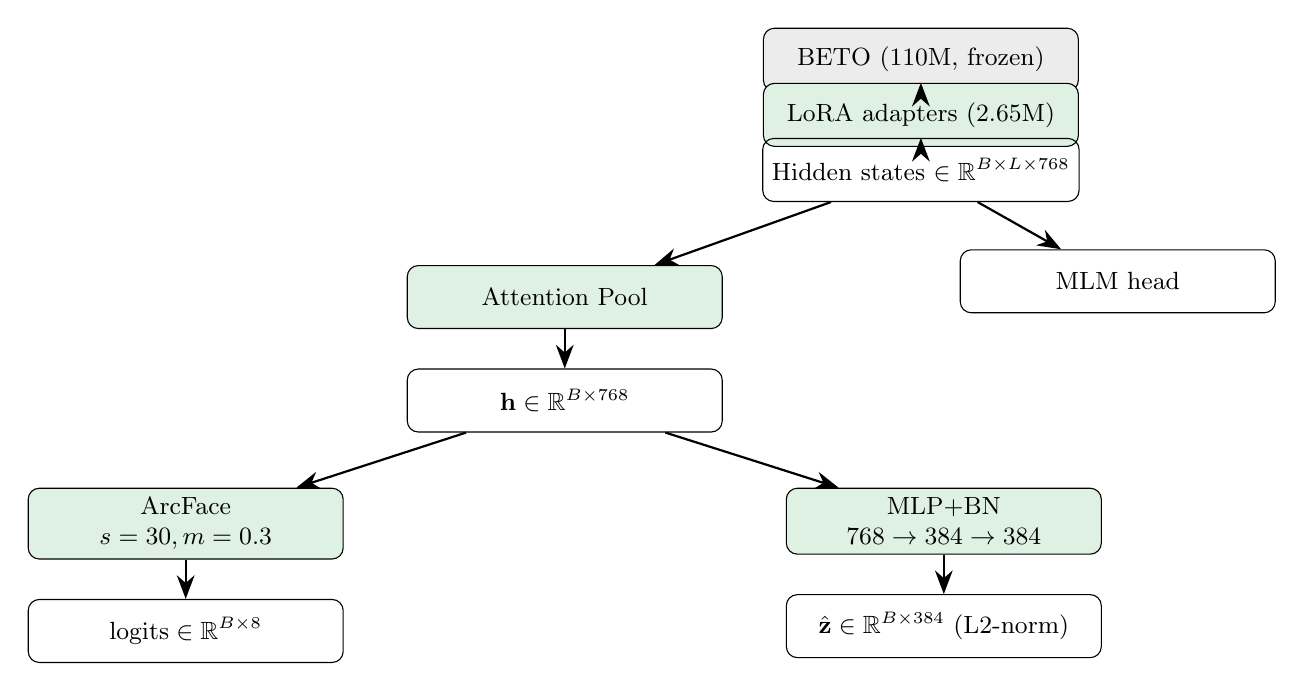
\begin{tikzpicture}[
    module/.style={rectangle, draw, rounded corners, minimum width=4cm, minimum height=0.8cm, align=center, font=\small},
    frozen/.style={module, fill=gray!15},
    train/.style={module, fill=v3color!15},
    arrow/.style={-{Stealth[length=3mm]}, thick},
    node distance=0.7cm
]
    \node[frozen] (beto) {BETO (110M, frozen)};
    \node[train, below of=beto] (lora) {LoRA adapters (2.65M)};
    \node[module, below of=lora] (hidden) {Hidden states $\in \R^{B \times L \times 768}$};
    \node[train, below left=0.8cm and 0.5cm of hidden] (pool) {Attention Pool};
    \node[module, below=0.6cm of hidden, xshift=2.5cm] (mlm) {MLM head};

    \node[module, below=0.5cm of pool] (pooled) {$\mathbf{h} \in \R^{B \times 768}$};

    \node[train, below left=0.7cm and 0.8cm of pooled] (arcface) {ArcFace\\$s=30, m=0.3$};
    \node[train, below right=0.7cm and 0.8cm of pooled] (proj) {MLP+BN\\$768 \to 384 \to 384$};

    \node[module, below=0.5cm of arcface] (cls) {$\text{logits} \in \R^{B \times 8}$};
    \node[module, below=0.5cm of proj] (emb) {$\hat{\mathbf{z}} \in \R^{B \times 384}$ (L2-norm)};

    \draw[arrow] (beto) -- (lora);
    \draw[arrow] (lora) -- (hidden);
    \draw[arrow] (hidden) -- (pool);
    \draw[arrow] (hidden) -- (mlm);
    \draw[arrow] (pool) -- (pooled);
    \draw[arrow] (pooled) -- (arcface);
    \draw[arrow] (pooled) -- (proj);
    \draw[arrow] (arcface) -- (cls);
    \draw[arrow] (proj) -- (emb);
\end{tikzpicture}
\end{center}

% ======================================================================
\section{Early Results: v1 vs v2 vs v3}
% ======================================================================

\subsection{Three-way comparison (first 2{,}000 steps)}

\begin{table}[H]
\centering
\caption{MLM loss trajectory across all three architectures.}
\label{tab:mlm_comparison}
\begin{tabular}{rccc}
\toprule
\textbf{Step} & \textcolor{v1color}{\textbf{v1 (GRL)}} & \textcolor{v2color}{\textbf{v2 (SupCon)}} & \textcolor{v3color}{\textbf{v3 (13 int.)}} \\
\midrule
200 & 10.41 & 10.40 & \textbf{10.28} \\
400 & 10.37 & 10.28 & \textbf{8.75} \\
600 & 10.30 & 9.14 & \textbf{7.72} \\
800 & 10.12 & 8.29 & \textbf{7.55} \\
1{,}000 & 9.30 & 7.83 & \textbf{7.49} \\
1{,}200 & 8.76 & 7.59 & \textbf{7.35} \\
1{,}400 & 8.33 & 7.52 & \textbf{7.18} \\
1{,}600 & 8.01 & 7.28 & \textbf{6.94} \\
1{,}800 & 7.76 & 7.03 & \textbf{6.63} \\
2{,}000 & 7.62 & 6.86 & \textbf{6.25} \\
\bottomrule
\end{tabular}
\end{table}

\begin{figure}[H]
\centering
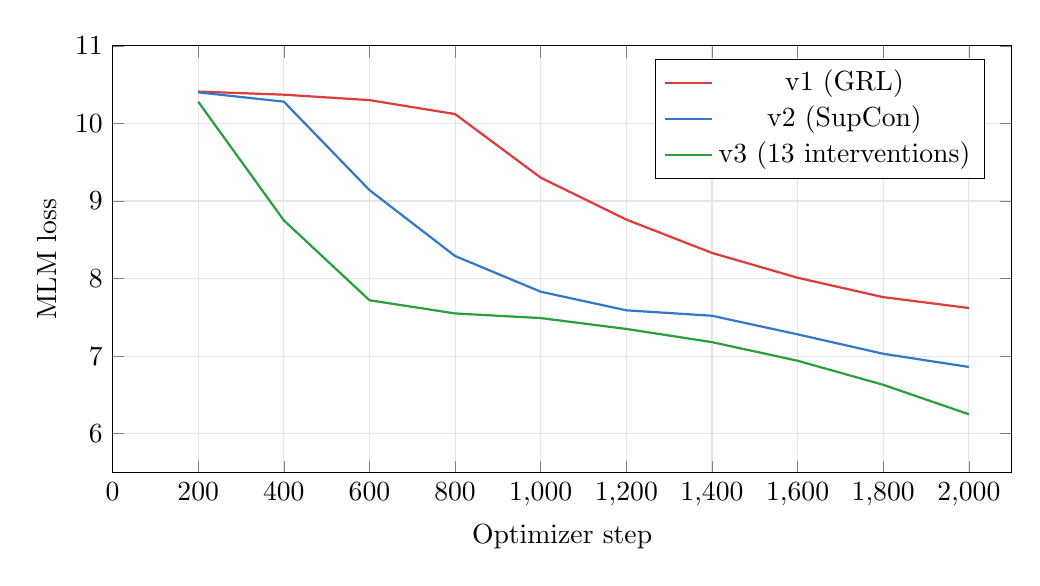
\begin{tikzpicture}
\begin{axis}[
    width=13cm, height=7cm,
    xlabel={Optimizer step},
    ylabel={MLM loss},
    xmin=0, xmax=2100,
    ymin=5.5, ymax=11,
    legend pos=north east,
    grid=major,
    grid style={gray!20},
]
\addplot[v1color, thick, mark=none] coordinates {
    (200,10.41) (400,10.37) (600,10.30) (800,10.12) (1000,9.30)
    (1200,8.76) (1400,8.33) (1600,8.01) (1800,7.76) (2000,7.62)
};
\addlegendentry{v1 (GRL)}

\addplot[v2color, thick, mark=none] coordinates {
    (200,10.40) (400,10.28) (600,9.14) (800,8.29) (1000,7.83)
    (1200,7.59) (1400,7.52) (1600,7.28) (1800,7.03) (2000,6.86)
};
\addlegendentry{v2 (SupCon)}

\addplot[v3color, thick, mark=none] coordinates {
    (200,10.28) (400,8.75) (600,7.72) (800,7.55) (1000,7.49)
    (1200,7.35) (1400,7.18) (1600,6.94) (1800,6.63) (2000,6.25)
};
\addlegendentry{v3 (13 interventions)}
\end{axis}
\end{tikzpicture}
\caption{MLM loss comparison. v3 learns fastest due to the pretrain phase
dedicating 100\% of gradient budget to MLM+CLS. At step 2{,}000: v3 is
0.6 nats below v2 and 1.4 nats below v1.}
\end{figure}

\subsection{Classification dynamics}

The classification losses are not directly comparable due to different
classifier architectures:

\begin{center}
\begin{tabular}{lccc}
\toprule
& \textbf{v1 (GRL)} & \textbf{v2 (SupCon)} & \textbf{v3 (13 int.)} \\
\midrule
Classifier type & Linear & Linear & ArcFace ($s$=30) \\
CLS at step 200 & 2.09 & 2.09 & 10.84 \\
CLS at step 2{,}000 & 2.03 & 1.73 & 2.90 \\
\midrule
Interpretation & Near-random & Learning & \textbf{Rapid angular sep.} \\
\bottomrule
\end{tabular}
\end{center}

v3's ArcFace CLS starts at $\sim$11 (due to $s = 30$ scaling and $m = 0.3$
margin) and descends steeply to 2.9 by step 2{,}000. The descent rate
($-4.0$/1{,}000 steps) is $4\times$ faster than v2's ($-0.2$/1{,}000 steps),
indicating that the 768-d pooled space is rapidly developing angular
separation between dialect clusters.

\subsection{Throughput}

\begin{center}
\begin{tabular}{lccc}
\toprule
& \textbf{v1} & \textbf{v2} & \textbf{v3} \\
\midrule
Samples/sec & 92 & 34 & 36 \\
MPS memory & --- & 1{,}794 MB & 1{,}794 MB \\
\bottomrule
\end{tabular}
\end{center}

v3 throughput is comparable to v2 (36 vs 34 sm/s). The additional
computation from BatchNorm, 2-layer MLP, and ArcFace is negligible.
v1 was faster because it used \texttt{max\_length=128} and LoRA on
only 3 targets; v2/v3 use \texttt{max\_length=256} and 6 LoRA targets.

% ======================================================================
\section{Predictions \& Verification Criteria}
% ======================================================================

\subsection{Expected timeline}

\begin{table}[H]
\centering
\caption{Predicted v3 loss trajectory at key milestones.}
\begin{tabular}{llcccc}
\toprule
\textbf{Milestone} & \textbf{Wall time} & \textbf{MLM} & \textbf{CLS} & \textbf{CON} & \textbf{CTR} \\
\midrule
End epoch 1 & $\sim$20h & $< 4.0$ & $< 1.5$ & 0 & 0 \\
End epoch 2 & $\sim$40h & $< 3.0$ & $< 1.0$ & 0 & 0 \\
Epoch 3, step 500 & $\sim$43h & $< 3.5$ & $< 1.2$ & $< 4.0$ & $> 0$ \\
End epoch 3 & $\sim$60h & $< 3.5$ & $< 1.2$ & $< 2.5$ & 0 \\
End epoch 4 (XBM on) & $\sim$80h & $< 3.0$ & $< 1.0$ & $< 2.0$ & 0 \\
End epoch 10 & $\sim$200h & $< 2.0$ & $< 0.5$ & $< 1.0$ & 0 \\
\bottomrule
\end{tabular}
\end{table}

\subsection{Red flags}

\begin{enumerate}
\item \textbf{Contrastive $> 5.0$ at end of epoch 3} --- the phase
transition has not occurred. Reduce $\tau$ to 0.05 and extend center
loss to 5{,}000 steps.

\item \textbf{Contrastive oscillates $> 3.0$ at epoch 5} --- XBM staleness.
Reduce XBM size to 2{,}048 or slow the ramp.

\item \textbf{MLM degrades after epoch 3} --- contrastive is corrupting
the base hidden states. Reduce $w_{\text{con\_final}}$ to 0.35.

\item \textbf{CLS plateaus $> 2.0$} --- ArcFace margin too aggressive.
Reduce $m$ from 0.3 to 0.15.
\end{enumerate}

\subsection{Success criteria}

The training is considered successful if:
\begin{enumerate}
\item $\loss_{\text{con}} < 2.0$ by end of epoch 5.
\item $\loss_{\text{con}} < 1.0$ by end of training.
\item Fisher discriminant ratio on the final $(V, 384)$ embeddings improves
over v2 for at least 6 of 8 varieties.
\item Downstream spectral eigenvalue gap (first vs second eigenvalue)
increases by $> 20\%$ compared to v2.
\end{enumerate}

% ======================================================================
\section{Preserved Artifacts}
% ======================================================================

All prior runs are preserved for comparison:

\begin{center}
\begin{tabular}{ll}
\toprule
\textbf{Directory} & \textbf{Contents} \\
\midrule
\texttt{outputs/eigen3\_v45\_grl\_baseline/} & v1 (GRL) run --- 21{,}521 steps \\
\texttt{outputs/eigen3\_v2\_supcon\_baseline/} & v2 (SupCon) run --- 21{,}600 steps \\
\texttt{outputs/eigen3/} & v3 (13 interventions) --- in progress \\
\texttt{outputs/embeddings/} & eigenv2 artifacts (untouched) \\
\texttt{outputs/v2\_real/} & eigenv2 real data outputs \\
\texttt{outputs/v2\_test/} & eigenv2 test outputs \\
\bottomrule
\end{tabular}
\end{center}

% ======================================================================
\section{References}
% ======================================================================

\begin{enumerate}[label={[\arabic*]}]
\item Khosla, P., et al. ``Supervised Contrastive Learning.''
\textit{NeurIPS}, 2020.

\item Wang, X., et al. ``Cross-Batch Memory for Embedding Learning.''
\textit{CVPR}, 2020.

\item Yeh, C.-H., et al. ``Decoupled Contrastive Learning.''
\textit{ECCV}, 2022.

\item Deng, J., et al. ``ArcFace: Additive Angular Margin Loss for Deep
Face Recognition.'' \textit{CVPR}, 2019.

\item Wen, Y., et al. ``A Discriminative Feature Learning Approach for
Deep Face Recognition.'' \textit{ECCV}, 2016.

\item Hu, E.J., et al. ``LoRA: Low-Rank Adaptation of Large Language
Models.'' \textit{ICLR}, 2022.

\item Ca\~{n}ete, J., et al. ``Spanish Pre-Trained BERT Model and
Evaluation Data.'' \textit{PML4DC at ICLR}, 2020.
\end{enumerate}

\end{document}
